\documentclass{article}
\usepackage[utf8]{inputenc}
\usepackage[german]{babel}
\usepackage{graphicx}
\usepackage[top=3cm, margin=1cm, bottom=3cm]{geometry}
\usepackage{hyperref}

\title{MTCG: Intermediate Protokoll}
\author{Rentenberger Lorenz}
\date{\today}

\begin{document}

\maketitle

\section{Projektübersicht}
Das Monster Trading Card Game (MTCG) ist eine REST-API Implementierung eines Kartenspiels. Die Anwendung ermöglicht Benutzern, sich zu registrieren, Karten zu sammeln, Decks zusammenzustellen und gegen andere Spieler anzutreten.

\subsection{GIT}
Link zum Github-Repository: \url{https://github.com/LRenTi/BIF3_SWEN1}

\section{Architektur und Design}
Die Architektur der Anwendung basiert auf einen mehrschichtigen Ansatz. Die API-Schicht (MTCG.Api) übernimmt die Bearbeitung von HTTP-Requests und das Routing der Endpunkte. Die Core-Schicht (MTCG.Core) enthält die Geschäftslogik und alle zentralen Entitäten des Spiels. Diese Trennung ermöglicht eine klare Struktur und erleichtert zukünftige Erweiterungen.

Ein wesentlicher Bestandteil des Designs ist die Implementierung einer sicheren Authentifizierung. Es wurde ein Token-basiertes System eingeführt, bei dem Tokens als zufällig generierte 24-stellige Zeichenketten erstellt werden. Diese Tokens werden in einem zentralen Speicher verwaltet, was eine effiziente und sichere Handhabung ermöglicht. Zusätzlich wurde für die Passwortsicherheit BCrypt verwendet, um die Passwörter der Benutzer zu hashen.

Zur Organisation der API-Endpunkte wurde ein flexibles Handler-System implementiert. Mithilfe von Attribut-basiertem Routing \textbf{[Route]} werden die Endpunkte definiert, während spezifische Handler wie UserHandler oder SessionHandler für die jeweilige Funktionalität zuständig sind. Dies ermöglicht eine klare Trennung der Logik und eine einfache Erweiterbarkeit. Das System ist durch die Einführung eines Interfaces für Handler flexibel gestaltbar und kann ohne großen Aufwand erweitert werden.

\section{Kartenspiel-Mechanik}
Die Kartenspiel-Mechanik bildet den Kern des Projekts. Karten werden in zwei Kategorien unterteilt: Monsterkarten und Zauberkarten. Die Karten verfügen über unterschiedliche Elementtypen wie Wasser, Feuer oder Normal, die ihre Effektivität in Kämpfen beeinflussen. Die Regeln für die Effektivität orientieren sich an klassischen Elementstärken (z. B. Wasser ist stark gegen Feuer). Jedes Deck ist auf vier Karten begrenzt, um strategische Entscheidungen der Spieler zu fördern und den Spielfluss zu verbessern.

\section{Herausforderungen und Lösungen}
Eine der größten Herausforderungen war die sichere Implementierung der Benutzerauthentifizierung. Hierfür wurde ein Token-basiertes System entwickelt, das es ermöglicht, API-Zugriffe eindeutig zu authentifizieren. Die Verwendung von BCrypt für das Hashing der Passwörter gewährleistet zusätzlichen Schutz vor unbefugtem Zugriff. Die zentrale Verwaltung der Tokens sorgt zudem für eine effiziente Verarbeitung und einfache Wartung.
Ein weiteres Problem war die Entwicklung einer strukturierten und erweiterbaren API. Dieses wurde durch ein handlerbasiertes System gelöst, das Attribut-Routing verwendet. Dadurch können neue Endpunkte leicht hinzugefügt werden, während die Trennung von Modellen und Data Transfer Objects (DTOs) die Übersichtlichkeit der Architektur bewahrt. Zudem wurden standardisierte API-Antworten eingeführt, um eine konsistente Kommunikation zwischen Server und Client zu gewährleisten.

\section{Klassendiagramm}
\begin{center}
    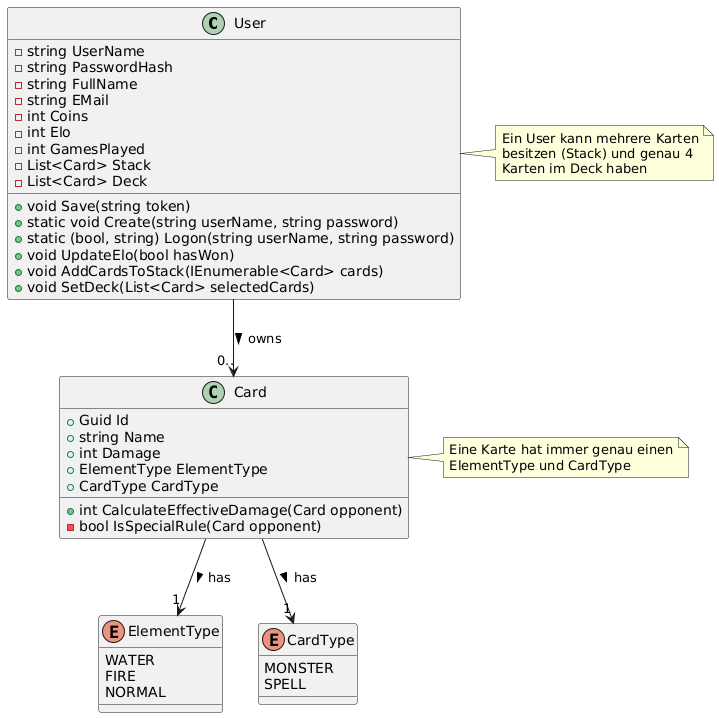
\includegraphics[width=0.5\textwidth]{UML.png}
    \label{fig:uml}
\end{center}


\end{document}